
\RequirePackage{cmap}

\documentclass[
    usenatbib,
]{mnras}

\usepackage[T1]{fontenc}
\usepackage[dvipsnames, x11names]{xcolor}

\renewcommand{\baselinestretch}{1.0} % Change to 1.65 for double spacing
\usepackage{showyourwork}
\usepackage{amsmath}
\usepackage{amsfonts}
\usepackage{amssymb}
\usepackage{mathrsfs}

\usepackage{xurl}
\urlstyle{tt}

\usepackage{booktabs}
\usepackage{graphicx}
\usepackage[
    % colorlinks=true, 
    % allcolors=blue,
]{hyperref}



\usepackage{libertine}
\usepackage[libertine]{newtxmath}
\usepackage[scaled=0.76]{beramono}
\usepackage{microtype}
\usepackage{csquotes}
\usepackage[capitalise]{cleveref}
%\usepackage{xspace}

\usepackage{standalone}
\usepackage{tikz}
\usetikzlibrary{
    calc,
    positioning,
    shapes,
}

\usepackage{siunitx}
\sisetup{
    range-units = single,
    range-phrase = {--},
    separate-uncertainty = true,
    multi-part-units = brackets,
    product-units = brackets,
    detect-weight = true,
    per-mode = symbol,
    mode = text,
}
\DeclareSIUnit\parsec{pc}
\DeclareSIUnit\au{au}
\DeclareSIUnit\mas{mas}

%REMOVE LATER
\usepackage{soul}

\usepackage{astro_bib_macro} %shortcuts of journals defined in this file

\newcommand{\todo}[1]{\textcolor{red}{[#1]}}
\newcommand{\timmy}[1]{\textcolor{red}{[\textbf{Timmy:} #1]}} % amazing

% Define macros
\newcommand{\IWA}{\ensuremath{\mathrm{IWA}}}
\newcommand{\hwo}{HabWorlds}

% Define the colors of the \rainbows
\definecolor{C0}{HTML}{ff0000}
\definecolor{C1}{HTML}{ff6d38}
\definecolor{C2}{HTML}{ecc86f}
\definecolor{C3}{HTML}{a4f89f}
\definecolor{C4}{HTML}{5af8c8}
\definecolor{C5}{HTML}{12c8e6}
\definecolor{C6}{HTML}{386df9}
\definecolor{C7}{HTML}{8000ff}

\newcommand{\rainbows}{%
    \textcolor{C0}{r}%
    \textcolor{C1}{a}%
    \textcolor{C2}{i}%
    \textcolor{C3}{n}%
    \textcolor{C4}{b}%
    \textcolor{C5}{o}%
    \textcolor{C6}{w}%
    \textcolor{C7}{s}%
    % \xspace
}

% Chasing rainbows with the Habitable Worlds Observatory
\title{Chasing \rainbows{} with the Habitable Worlds Observatory}
%Scattering phase angle probed by directly imaged planets, or
%Don't ask us about contrast


% Authors are in alphabetical order:
\author[Sophia R. Vaughan et al.]{%
    Sophia R. Vaughan$^{1,}$\thanks{Correspondence:  \url{sophia.vaughan@physics.ox.ac.uk}}
    Kimberly Bott$^{2,9}$,
    Sarah L. Casewell$^{3}$,
    Nicolas B. Cowan$^{4}$,
    David S. Doelman$^{5}$,\newauthor
    Timothy D. Gebhard$^{6}$,
    Matthew Kenworthy$^{5}$,
    Johan Mazoyer$^{7}$,
    Maxwell A. Millar-Blanchaer$^{8}$
    \newauthor [remaining workshop participants in alphabetical order] \newauthor 
    \\
    $^{1}$ Department of Astrophysics, University of Oxford, Denys Wilkinson Building, Keble Road, Oxford OX1 3RH, UK\\
    $^{2}$ Department of Earth and Planetary Sciences, University of California, Riverside, CA 92521, USA \\
    $^{3}$ Centre for Exoplanet Research, School of Physics and Astronomy, University of Leicester, University Road, Leicester, LE1 7RH, UK\\
    $^{4}$ Department of Earth \& Planetary Sciences and Department of Physics, McGill University, 3600 rue University, Montréal, QC, H3A 2T8, Canada\\
    $^{5}$ Leiden Observatory, Leiden University, P.O. Box 9513, 2300 RA Leiden, The Netherlands\\
    $^{6}$ Max Planck Institute for Intelligent Systems, Max Planck Ring 4, 72076 Tübingen, Germany \& ETH Zurich, Switzerland \\
    $^{7}$ LESIA, Observatoire de Paris, Université PSL, CNRS, Sorbonne Université, Université de Paris, F-92195 Meudon, France \\
    $^{8}$ Department of Physics, University of California, Santa Barbara, CA 93106, USA \\
    $^{9}$ NASA Nexus for Exoplanet System Science, Virtual Planetary Laboratory Team, Seattle, WA 98195, USA
}
\date{Draft version: \today}


\pagestyle{plain}
 
\begin{document} 

\maketitle

\begin{abstract}
NASA recently announced the Habitable Worlds Observatory, a coronagraphic mission which would detect rocky planets in the habitable zone, establish their habitability, and search them for biosignatures. 
%Numerous instrumental and observational challenges have still to be overcome to design a coronagraphic mission with that goal. After a research phase aiming at the detection of a few tens of exo-Earth in the habitable zone, the Habitable Worlds Observatory will use its spectroscopic and polarimetric capabilities to probe these planets' atmosphere and surface properties. 
Surface liquid water is central to the definition of planetary habitability.
%
Photometric and polarimetric phase variations can show the presence of specularly reflecting oceans on exoplanets, in addition to being sensitive to rainbows and other cloud scattering effects. Direct imaging missions are optimised to detect planets near quadrature, which may obscure some of the phases at which these features are strongest. The range of scattering phases accessible for an exoplanet can be limited by its orbital inclination or the coronagraph's inner working angle. Planets that orbit close to edge-on have accessible phase angles limited by obscuration by the coronagraph. We use the list of target stars for the Habitable Worlds Observatory to estimate the number of exo-Earths that could be searched for non-Lambertian scattering phenomena. We find that exo-Earths in systems listed in this Habitable Worlds Observatory catalog will have a detectable Rayleigh scattering peak. The glint signature at scattering phases of $\sim$50--70$^\circ$ would be accessible to the Habitable Worlds Observatory in $\sim$20 systems, and the rainbow of water clouds at phases of 140--160$^\circ$ would be accessible in $\sim$55 systems, assuming a 60 mas inner working angle (\IWA). The number of systems in which an exo-Earth could be searched for these scattering phenomena increases with orbital eccentricity and scales approximately inversely with \IWA.       


\end{abstract}

\begin{keywords}
planets and satellites: terrestrial planets -- instrumentation: high angular resolution -- planets and satellites: atmospheres
\end{keywords}

%%%%%%%%%%%%%%%%%%%%%%%%%%%%%%%%%%%%%%%%%%%%%%%%%%%%%%%%%%%%%%%%%%%%%%%%%%%%%%%%%%%%%%%%%%%%%%%%%%%%%%%%%%%%%%%%%%%%%%%%%%%%%%
\section{Introduction}
\label{sec:intro}

\begin{figure*}%[t]
   \centering
   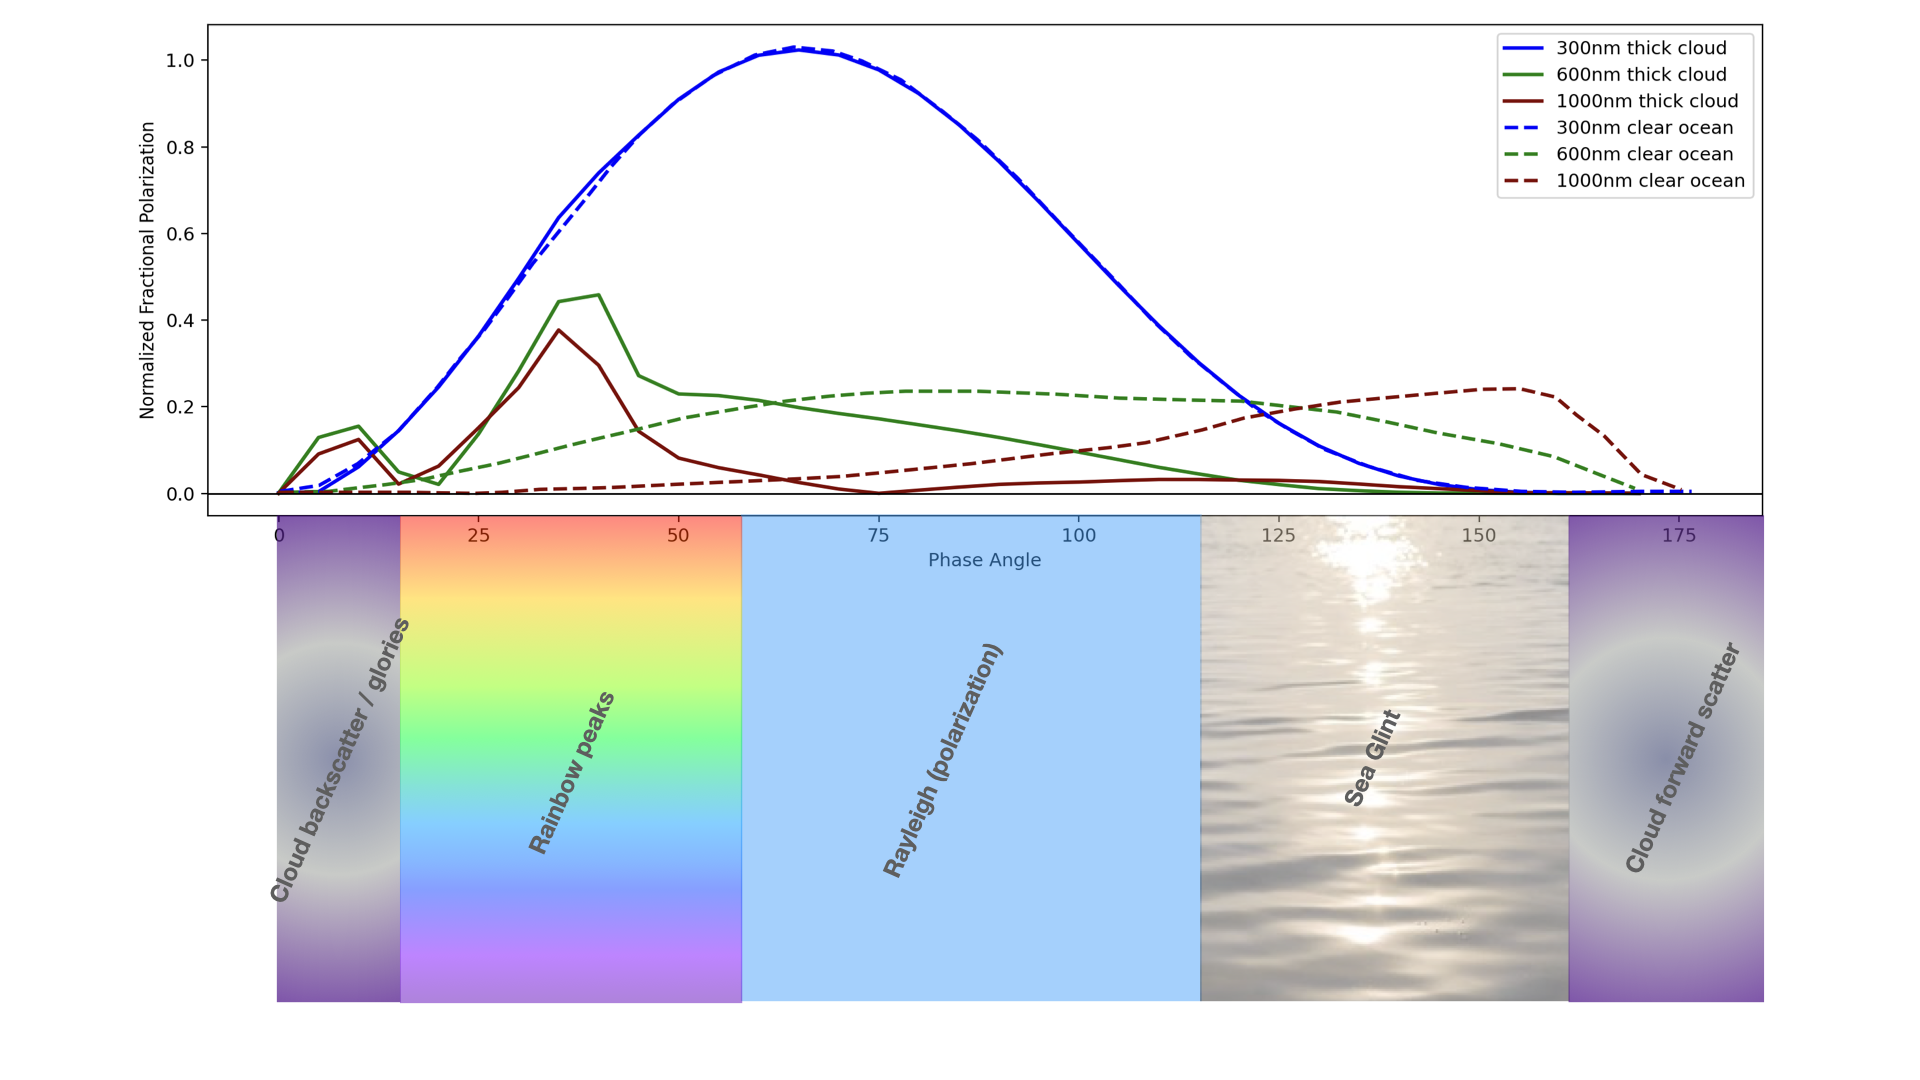
\includegraphics[width=\linewidth]{figures/Fig1IWAPol.png}
   \caption{BOTT PLOT this is a holder until Kim updates the figure}
    \label{fig:bottplot}
\end{figure*}

%\textcolor{red}{introduce motivation, specs for habitable worlds observatory and the document we got the target list from.}


Surface liquid water is closely related to planetary habitability: water is required for life as we know it, and life on exoplanets will most likely on be detectable if it is present at the surface. 

To first order, the presence of surface liquid water can be predicted by the flux a planet receives from its star. The habitable zone (HZ) describes the range of semi-major axes around a given main sequence star for which an Earth-like planet could maintain surface liquid water \citep{kasting93}.  The HZ is convenient because a planet can be deemed habitable based on solely on its orbital separation, but it remains an untested hypothesis. %Ideally, we will empirically establish the presence of liquid water on an exoplanet before trying to interpret its putative biosignatures.  

%\textcolor{blue}{Kim will enhance the polarimetry stuff, and we should break into multiple paragraphs.}\\

%\textbf{Why glint [Kim]}
% probe of surface conditions; habitability

\subsection{Ocean Glint}
\cite{2001Natur.412..885F} noted the potential for time-resolved photometry to identify water oceans on the surface of an exoplanet, which was further explored by \citet{williams2004} and \citet{giados2006}. Rotational variability of an exoplanet's reflected light colours can be inverted into a rough map of the planet's surface, with dark regions being suggestive of oceans \citep{2009ApJ...700..915C}, but specular reflection, a.k.a. glint, remains the most direct means to infer liquids on the surface of other worlds \citep[e.g., methane lakes on Titan;][]{2010GeoRL..37.7104S}. \citet{lustig2019} explored mapping exoplanets from their ocean glint in polarized light.

In polarized light the glint appears at similar phase angles but its peak can be extended further particularly in the presence of atmospheric winds \citep{kopparla2018}.
%\cite{2006astro.ph.10518M} quantified how photometric and polarimetric scattered light orbital phase variations might betray the presence of oceans on terrestrial exoplanets.  
\citet{Takahashi2021} used polarimetric Earthshine measurements to detect the presence of the ocean.
\cite{2008Icar..195..927W} simulated photometric and polarimetric phase curves of directly imaged terrestrial planets. They noted that surface oceans would be detectable because they are more reflective and exhibit a peak in polarization at crescent phases. 

% NEEDS Paragraph on mapping connection to tectonics

% NEEDS KOPPARLA (prob refer to , BERDYUGINA, ROSSI? (cloud?), HU?, added... blend cloud hinderance into argument for context to lead into rainbows, mention Lietzow and jeremy there., maybe some more mention of the Earthshine observations Karalidi, Gordon, etc

%"Stam & Hovenier (2006) independently examined the observability of the polarized signatures of an Earth-like extrasolar planet, including Rayleigh scattering and sea-surface glint. Schneider (2006) had similar ideas." -KB


% Move to Clouds?
In practice, clouds complicate the detection of ocean glint because they obscure the underlying surface and can act as strong forward scatterers, mimicking ocean glint. \cite{2010ApJ...721L..67R} compared observations of the Earth's scattering phase curve to radiative transfer simulations; they found that the photometric brightening of Earth at crescent phases is mostly due to forward scattering from clouds, with a relatively small contribution from ocean glint.
\cite{Zugger_2010} simulated photometric and polarized phase variations for Earth-like planets including the effects of partial cloud coverage in suppressing the Rayleigh scattering and ocean glint polarization. Although the presence of clouds and atmospheric Rayleigh scattering weaken the signal of an underlying ocean, they again find that oceans are detectable and distinguishable from other sources of polarization. To suppress the effects of Rayleigh scattering, glint observations can be made at longer wavelengths
\citep{Zugger_2011}. 



%%% KIM's BOOKMARK FOR HERLSELF, PLEASE DO NOT DELETE %%%


\subsection{Polarized Phase Curves}
%compare to features in nonpol (strength rainbow); current capabilties?, errors from 3 papers, 

% add latitude albedo degeneracy break here \citep{2012ApJ...752L...3C}

%This has the added advantage of minimizing the latitude--albedo effect, which could otherwise be a false-positive for photometric brightening at crescent phases due to glint \citep{2012ApJ...752L...3C}. 

 %\cite{2019A&A...626A.129T,2022A&A...664A.172T} simulated the photometric and polarimetric signatures of terrestrial planets with inhomogeneous clouds.

 Phase curves of planets are more complex than simple Lambertian curves.
 %
 The phase curve of an edge on system in unpolarized light is dominated by the reflectance and backscatter of the surface, clouds, and atmosphere.
 %
 Though this behaviour is not Lambertian, the planet will, in general, get brighter at fuller phases (small scattering angles) with a peak at full phase from cloud backscatter \citep[see, for example,][]{kopparla2018}.
 %
 In cases where surface liquid (sea) is present, the specular reflection can create a notable addition to the phase curve at broad scattering angles near crescent phase \citep{Robinson_2010}.
 %
 Exoplanet phase curves can also contain a rainbow signature at gibbous phases (moderately narrow scattering angles), though this is a small feature in comparison to the reflectance.

 In polarized light, additional structure in the phase curve can enable phenomena like ocean glint, rainbows, and the Rayleigh scattering to be more easily distinguished.  Notably, in the polarized phase curve the rainbow may be an especially strong feature and the maximum reflectance signal (from Rayleigh scattering) occurs 

 


%Polarimetry provides the possibility to detect molecules, hazes, clouds and different surfaces  as they all produce unique polarization signatures which cannot be disentagled by using broadband flux alone. Polarized measurements of terrestrial exoplanet atmospheres therefore have the potential to provide empirical constraints on atmospheric properties that are inaccessible through other observational techniques. Polarimetry has previously played an important role in the understanding of solar system planet atmospheres, for instance, polarimetric measurements of Venus’ atmosphere suggested that the upper atmosphere of Venus is dominated by a haze of liquid sulphuric acid droplets \citep{Venus74}, which has been confirmed by in situ observations.

\subsection{Rainbows}
%calc; retrieve species including for non terrestrials; droplet liklihood of liquid surface; lit review bailey et below

%The rai


%cloud coverage paper in polarisation :
%\cite{rossi17} computed flux and polarisation of reflected starlight for different types of cloud cover on Earth-like planets and determined different types of cloud cover can be distinguished from each other. %Alternative options or papers here.... Kim can write this tomorrow , needs other Stam, Karalidi, Kopparla, maybe Gordon, need to reference rainbows in Bailey paper.  Look at citations in Gordon paper (our bib)... he has a really thorough lit review --KB


The National Academy of Sciences Astronomy \& Astrophysics 2020 Decadal Survey \citep{decadal} recommended the first in a new \enquote{Great Observatories} program a telescope with the capability to detect signatures of habitability for about 25 habitable zone planets.
%
This assertion requires an instrument with a coronograph capable of high contrast imaging in the optical-near infrared.
%
Following this release, NASA recently announced the start of the development of the Habitable Worlds Observatory (\hwo).
%
The precursor technology recommended by the Decadal Survey also lists ``direct imaging to probe polarized ocean glint on terrestrial planets'' as one of the priority capabilities \citep[Box E.1 in][]{decadal} for ground and space-based observatories.
%
The performance and precise characteristics of this telescope (on-axis or off-axis, exact diameter, type of segmentation, type of coronagraph) are still to be determined.
%
The development will be heavily influenced by the LUVOIR \citep{LUVOIR2019} and HabEx \citep{HabEx_2020} preparatory studies.
%
The Inner Working angle (\IWA) of the resulting telescope will be dependent on these choices, which in turn will have a significant impact on the expected exo-Earth yield \citep{Stark2019_exoplanetyield}.

Extreme Coronagraph for Living Planetary Systems (ECLIPS) coronograph for LUVOIR was a proposed \SIrange{200}{2000}{\nano\meter} instrument for exoplanet characterisation, with a similar coronagraph operating between \num{450} and \SI{1800}{\nano\meter} planned for HabEx.
%
POLLUX, a proposed UV instrument for the LUVOIR study could also allow the detection of polarised light from hot Jupiters at \SI{300}{\nano\meter} \citep{Bouret2018_pollux}.
%
However, the challenges associated with the design of a coronagraph in UV are enormous, and it is unlikely that \hwo will include a UV high-contrast instrument sensitive to Earth-like planets.


%We ignore contrast in this study
%OWA -> should go in discussions




%\textbf{In this paper we...}
In this paper we quantify the accessible scattering phase angles for hypothetical terrestrial planets orbiting in the habitable zones of HabWorlds target stars. In \S 2.1 we describe the target list, in \S 2.2 we derive expressions for the range of scattering phase angles in a few different limits, in \S 2.3 we describe Monte Carlo simulations to marginalize over the unknown orbital inclination and eccentricity of planets in these systems, and in \S 2.4 we outline how the planet/star contrast changes as a function of orbital phase.  We present and discuss our results in \S 3 and conclude in \S 4.  %the   the way that inclination and coronagraph inner working angle can limit the accessible phase angles  
% We minimally explore the contrast ratio as we are primarily exploring whether these scattering angles are reachable with inner working angle and outer working angle considered.

% We do not consider the particulars of specific planet scenarios as that work is completed by foward models

%We do not separate Stokes parameters as we are interested in where the net signal is achievable with IWA and OWA. 



%%%%%%%%%%%%%%%%%%%%%%%%%%%%%%%%%%%%%%%%%%%%%%%%%%%%%%%%%%%%%%%

%\section{Plots to Include}
%\label{sec:plots}
%\begin{enumerate}
%    \item \st{Cartoon defining various phase angles: orbital phase, scattering phase, $\beta$ ? (Sophia)}
%    \item Bott plot: annotated polarized and unpolarized phase curves for ocean world and cloudy worlds (Kim)
%    \item \st{3x3 cartoon showing effect of inclination and IWA compared to orbit (Sophia)}
%    \item Cumulative distribution functions, both simple (circular, edge-on), bit more realistic (circular, but range of inclinations), and full-on (range of inclinations and eccentricities). Max \& Matthew
%    \item Scatter plot of stellar effective temperature vs system distance (Timmy)
%\end{enumerate}
 
%%%%%%%%%%%%%%%%%%%%%%%%%%%%%%%%%%%%%%%%%%%%%%%%%%%%%%%%%%%%%%%%%%%%%%%%%%%%%%%%%%%%%%%%%%%%%%%%%%%%%%%%%%%%%%%%%%%%%%%%%%%%%%

%\section{Observing scattering phenomena}
\section{Methods}

%%%%%%%%%%%%%%%%%%%%%%%%%%%%%%%%%%%%%%%%%%%%%%%%%%%%%%%%%%%%%%%

\subsection{\hwo\ and Stellar Sample}
%\textcolor{blue}{Merge the 2 sections here into "Assumed technical specifications and sample"? I don't think this needs to be 2 subsections}
\hwo\ is still in the early stages of development, and the exact telescope and instrument design is undecided. 
%
In this work, we assume a \SI{6}{\meter} primary mirror, which is the currently favoured design for the observatory.
%
In addition, the observatory will utilise a coronagraph to suppress the stellar light and facilitate high contrast observations of their faint exoplanet companions. 
%
The \IWA\ of the coronagraph is currently undecided and will be driven by both the science requirements and technological limitations. 
%In this work, we investigate the scattering phase coverage obtainable for several choices for the \IWA\ of the observatory. 
%We also consider the Outer Working Angle (OWA) but for most targets this is not a limiting factor. 
For ease of comparison, \cref{tab:IWA_OWA} indicates the angular separations corresponding to multiples of $\lambda / D$ for a \SI{6}{\meter} telescope at a wavelength of $\lambda = \SI{-1}{\nano\meter}$ \todo{Update value!}.

\begin{table}
    \centering
    \caption{
        Conversion between $\lambda / D$ and \si{\mas} for different wavelengths, assuming $D = \SI{6}{\meter}$. 
        \todo{We should use consistent wavelengths for this table, for the Bott Plot, and for the M\&M cumulative distribution function. Also update to use the only wavelength we choose.}
    }
    \label{tab:IWA_OWA}
    \begin{tabular}{ c c c c } 
    \toprule
     & $\lambda/D$ & mas (at \SI{600}{\nano\meter}) & mas (at \SI{700}{\nano\meter}) \\
    \midrule
    \midrule
    IWA & 1 & 20.63 & 24.06 \\
    IWA & 2 & 41.25 & 48.13 \\
    IWA & 3 & 61.88 & 72.19 \\
    IWA & 4 & 82.51 & 96.26 \\
    \midrule
    OWA & 32 &  660.05 & 770.06 \\
    OWA & 64 & 1320.09 & 1540.11 \\
    \bottomrule
    \end{tabular}
\end{table}


\hwo\ is currently envisioned to observe the stars stated in the NASA Exoplanet Exploration Program's Mission Star List for the Habitable Worlds Observatory.%
\footnote{\url{https://exoplanets.nasa.gov/internal_resources/2645_NASA_ExEP_Target_List_HWO_Documentation_2023.pdf}}
%
This list comprises $\sim$160 stars, the majority of which are Sun-like dwarfs; 66~F~dwarfs, 55~G~dwarfs, 40~K~dwarfs, and 3~M~dwarfs.
%
The target list is constructed assuming a maximum planet magnitude of $R_c = 31$ and a contrast floor of \num{2.5e-11}. 
%with an occurrence rate of rocky planets in the optimistic habitable zone to be $\eta_{\oplus}$ = 0.24 \citep{decadal}. 
The corresponding adopted habitable zone limits are a semi-major axis of \SIrange{0.95}{1.67}{\au} for a solar twin, planet sizes between \SIrange{0.8}{1.4}{} Earth radii, and for non-solar stars, scale as square root of the bolometric luminosity normalized to the Sun. 
%
This range of orbital separation corresponds to the \enquote{conservative habitable zone} \citep{kasting93, kopparapu13}. 
The authors of the report determined that these are the nearby stars (maximum distance \SI{25}{\parsec}) for which exo-Earths would be the most observable for an imaging survey of habitable zones with a \SI{6}{\meter} telescope. 

In what follows, we consider hypothetical Earth-size planets orbiting at the right distance from each star to receive the same flux as the Earth receives from the Sun. By construction, such planets should be observable at quadrature phase by HabWorlds. 

%%%%%%%%%%%%%%%%%%%%%%%%%%%%%%%%%%%%%%%%%%%%%%%%%%%%%%%%%%%%%%%

\subsection{Maximum scattering phase angle coverage}
\label{sec:Delta_phi}

The coronagraph can obscure part of the planet's orbit which, as demonstrated in \cref{fig:annotated-orbit}, can prevent the planet from being observed at high and low scattering angles. 
%
The range of scattering phase angles that can be observed will depend on the \IWA\ of the coronagraph as well as the shape and orientation of the exoplanet's orbit.

\begin{figure}
    \centering
    \includestandalone{tikz/annotated-orbit}
    \caption{
        The coronagraph can obscure the exoplanet at high and low scattering phase angles. This can prevent observations of scattering phenomena which could be used to indicate the habitability and atmospheric composition of the exoplanet. \todo{Add why scattering is cool} 
    }
    \label{fig:annotated-orbit}
\end{figure}

%%%%%%%%%%%%%%%%%%%%%%%%%%%%%%%%%%%%%%%%%%%%%%%%%%%%%%%%%%%%%%%

\subsubsection{Circular edge-on orbits}

In the non-eccentric case (i.e., with a circular orbit and where the coronagraphic mask centred on the star), minimum ($\varphi_\mathrm{min}$) and maximum ($\varphi_\mathrm{max}$) scattering phase angles accessible are symmetric about 90 degrees. 
%
We define the angle $\Delta \varphi$ such that: 
\begin{equation}
    \label{eq:Delta_phi}
    \Delta \varphi 
    = \varphi_\mathrm{max} - \varphi_\mathrm{min}
    =  2(\varphi_\mathrm{max} - 90) 
    =  2(\varphi_\mathrm{min} + 90)
\end{equation}

The on-sky projected planet distance, $r_\mathrm{proj}$ (in \si{\au}) is shown in \cref{fig:scattering-angle} assuming a non-eccentric circular orbit with a semi-major $a$ (in \si{\au}) at a distance $d_*$ (in \si{\parsec}) from the observer. 
%
The scattering phase angle $\varphi$ is this set up follows the equation,
\begin{equation}
    \sin(\varphi) = \frac{r_\mathrm{proj}}{a}
\end{equation}
%
Using small angles, $r_\mathrm{proj} = \delta d_*$ where $\delta$ is the angular separation on-sky.
%
We access the minimum scattering angle when the projected distance reaches the inner working angle separation $\delta = \mathrm{IWA}$. 
%
Using \cref{eq:Delta_phi}, we deduce:

\begin{equation}
    \label{eq:scattering_angle}
    \cos\left(\dfrac{\Delta \varphi}{2}\right) = \frac{\mathrm{IWA \cdot d_*}}{a}
\end{equation}
 
\begin{figure}
    \centering
    \includestandalone{tikz/scattering-angle}
    \caption{
        The on-sky projected planet distance, $r_\mathrm{proj}$, of a planet with a semi-major $a$ at a distance $d_*$. The on-sky angular separation as viewed by the observer is $\delta$. The scattering phase angle, $\varphi$, is the angle between the line of sight to the star and the line connecting the star and planet.  
    }
    \label{fig:scattering-angle}
\end{figure}

\Cref{fig:scatterplot} shows $\Delta \varphi$ for the systems in the HabWorlds target list assuming an IWA of 62 mas ($3 \lambda / D$ coronagraph at $\SI{600}{\nano\meter}$). 
%
%This assumes each planet has a semi-major axis such that it receives an Earth-equivalent instellation, which is provided in the input star list.
%
For edge-on circular orbits, it will be possible to observe Rayleigh scattering for all targets and rainbows will be accessible in some cases.

\begin{figure*}
    \centering
    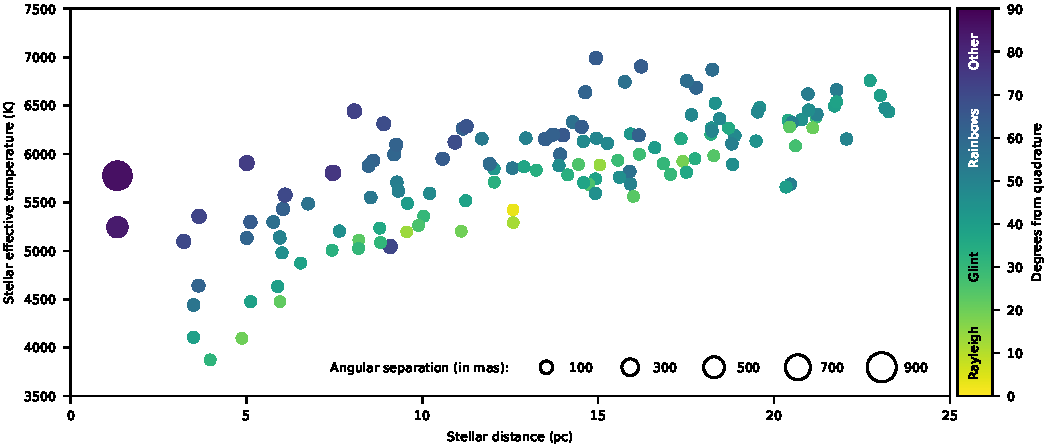
\includegraphics{figures/scatterplot.pdf}
    \caption{
        \timmy{I believe those should be the results for circular, edge-on orbits, but let's double-check with Max.}
        Scatter plot at 3 $\lambda/D$ for the target sample, showing stellar effective temperature and stellar distance. 
        The size of the points represents the angular separation of the star and planet in milliarcseconds as presented in the target list. 
        The colour of the points shows the atmospheric phenomenon that can be detected with darker colours, including all lighter (yellow) colour phenomenon. 
        Thus, dark blue points are systems which have the most key features, as systems in which the angles required to see the rainbow are probed will also have the angles required to see the Rayleigh scattering probed.
    }
    \label{fig:scatterplot}
    \script{create-scatterplot.py}
\end{figure*}

%%%%%%%%%%%%%%%%%%%%%%%%%%%%%%%%%%%%%%%%%%%%%%%%%%%%%%%%%%%%%%%

\subsubsection{Circular inclined orbits}

Most systems will not be viewed as edge on from Earth.
%
For a given system with inclination $i$, we have identified 2 regimes, which are shown in \cref{fig:orb-grid}:

(1)~If the inclination is relatively face-on, then the coronagraph mask does not obscure any part of the sky-projected orbit, and the maximum scattering phase angle coverage depends solely on the disk inclination ;

(2)~When parts of the orbit  are hidden by the focal plane mask, the scattering phase angle coverage only depends on the \IWA\ and orbital semi-major axis. 

\begin{figure}[htb]
   \centering
   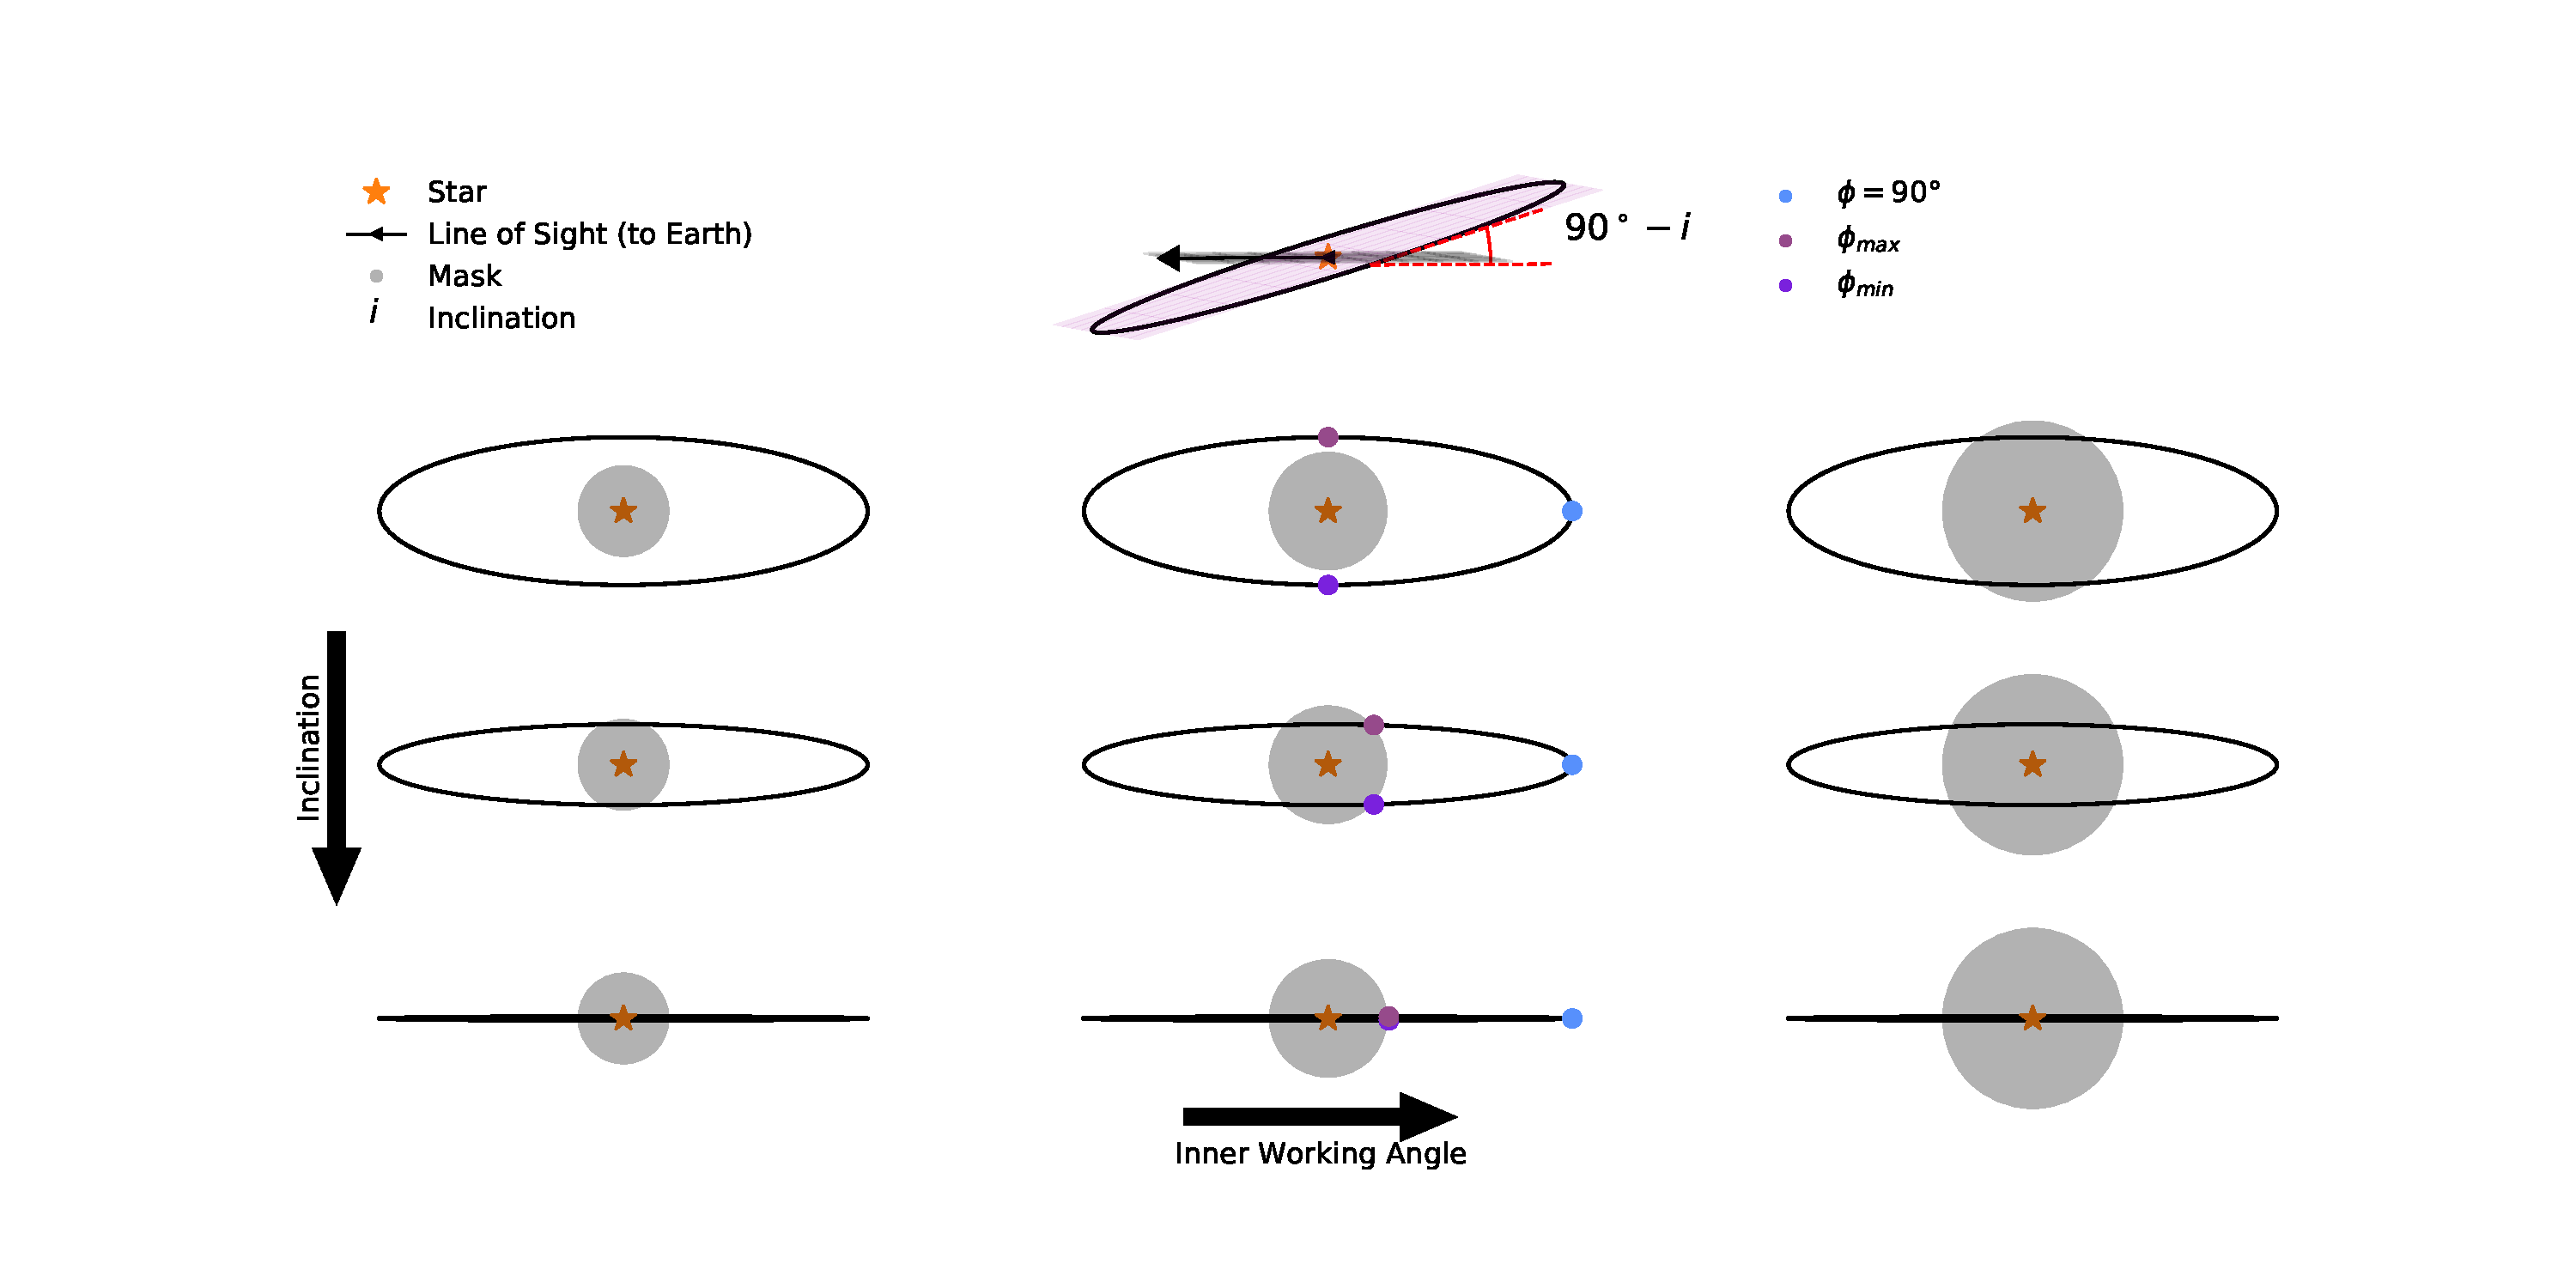
\includegraphics[width=0.99\columnwidth]{figures/orb-grid.pdf}
   \caption{
        The scattering phase angles accessible to a direct imaging mission can be limited by orbital inclination or by the coronagraphic inner working angle. 
        If the orbital inclination is close to face-on (top panels) then the scattering phase angles probed throughout an orbit are limited by inclination; for circular orbits accessible scattering phases are $\phi \in 90^\circ \pm i$. 
        For orbital inclinations close to edge-on (bottom panels) the planet goes through all phases, but the scattering phase angles near 0$^\circ$ and 180$^\circ$ are not accessible due to obscuration by the coronagraph mask; for circular orbits, the accessible scattering phases are $\phi \in 90^\circ \pm \arcsin({\rm IWA}\cdot d_*/a)$.
    }
    \label{fig:orb-grid}
    \script{plot-orb-grid.py}
\end{figure}

Using \cref{eq:scattering_angle}, we deduce the equation for inclined circular orbits: 
\begin{equation}
\label{eq:Delta_phi_max}
    \Delta \varphi = 
    \begin{cases}
        2 \cdot i & \textrm{for} \cos(i) > \dfrac{\mathrm{IWA}\cdot d_* }{a}
  \\ 
        2 \cdot \cos^{-1}\left(\dfrac{\mathrm{IWA}\cdot d_* }{a}\right)  & \textrm{for} \cos(i) < \dfrac{\mathrm{IWA}\cdot d_* }{a}
    \end{cases}\,.
\end{equation}

%%%%%%%%%%%%%%%%%%%%%%%%%%%%%%%%%%%%%%%%%%%%%%%%%%%%%%%%%%%%%%%

%\subsubsection{Eccentric orbits}


%The inclination $i$ is sampled such that $\cos(i)$ follows a uniform distribution, $\cos(i) \sim \mathcal{U}(0, 1)$.

%%%%%%%%%%%%%%%%%%%%%%%%%%%%%%%%%%%%%%%%%%%%%%%%%%%%%%%%%%%%%%%
\subsection{Monte Carlo Simulations}

\subsubsection{Circular randomly inclined orbits}
\label{sec:circular}

For each star on the \hwo\ target list, we generate XX hypothetical habitable planets at the Earth-equivalent-flux semi-major axis. 
%
The orbital inclinations are randomly drawn from a distribution uniform in $\cos i$. 
%
We then use \cref{eq:Delta_phi_max} to determine the range of accessible scattering phase angles for each hypothetical planet. 
The solid lines in Figure \ref{fig:betaallofit} show the cumulative distribution for the most extreme scattering phase angles accessible for the \hwo\ target list, depending on the choice of inner working angle.  

\todo{what does this plot show, how many systems could we see?}

%%%%%%%%%%%%%%%%%%%%%%%%%%%%%%%%%%%%%%%%%%%%%%%%%%%%%%%%%%%%%%%

\begin{figure*}[t]
    \centering
    \includegraphics[width=0.95\textwidth]{figures/accessible_phase_angles.png}  
    \caption{
        The big kahuna
        \timmy{What are the dashed vs. solid lines?}
        \timmy{How did this plot aggregate the simulations for each planet? mean? median? min/max?
        }
    }
    \label{fig:betaallofit}
    \script{plot_n_versus_phase.py}
\end{figure*}

\subsubsection{Eccentric randomly inclined orbits}
\label{sec:eccentric}
We repeat the Monte Carlo simulation from \cref{sec:circular} assuming the orbital eccentricity follows a beta distribution with shape parameters $a=0.867$ and $b=3.03$ \citep{2013MNRAS.434L..51K}. 
%
We randomly drew 1000 random orbits for each star and determined the sky-projected orbits following, e.g., \cite{2010exop.book...15M}. Eccentricities were drawn from the beta distribution, and inclinations were uniform in $\cos i$. 
%
We then filtered on \IWA's of 1, 2, 3 and 4 times $\lambda / D$, before identifying which targets would be observable at the scattering phase angles where ocean glint, rainbows, or the Rayleigh peak occur. 
%
\Cref{fig:ball-o-yarn} shows a sample of the generated orbits with the filtered \IWA's. The dashed lines in Figure \ref{fig:betaallofit} show the cumulative distribution for the most extreme scattering phase angles accessible, when accounting for orbital eccentricity.  Kepler's second law ensures that eccentric planets spend more time at orbital separations greater than their semi-major axis, and hence are more likely to peak out from behind the coronagraph IWA and extreme orbital phases (albeit with worse contrast due to the greater star--planet separation). 

\todo{how was the angle coverage calculated in the monte carlo?}

%
%Each plot has been scaled such that the habitable zone occupies the same radius, hence the \IWA's vary in apparent size compared to the orbit. 

\subsection{Simulating contrast curves}
\textbf{Kim and David}
%
A second parameter that is crucial for detecting features like rainbows and ocean glint on Earth-like planets is the contrast, i.e. the relative flux of the reflected light from the planet divided by the stellar flux. 
%
While this is not the main focus of this paper, it is important to consider that the contrast and polarised contrast are not constant as function of scattering phase angles.
%
This is due to a combination of the changing illumination fraction of the exoplanets Earth facing surface and scattering effects.
%
Here, we aim to present some simplified examples of the impact of the scattering angle dependent contrast on the detectability of rainbow and glint features. 
%
We note that these calculations are by no means complete or exact, given the many variables that go into modelling reflected fluxes and polarization fractions of an Earth-like planet \citep{ treesstam2019,trees2022}.


The NASA Exoplanet Exploration Program’s Mission Star List for the Habitable Worlds Observatory includes an estimated contrast ratio for an Earth twin in the habitable zone for every star. 
%
The contrast is calculated as 
\begin{equation}
C = F_p/F_* = p \phi (\alpha) (R_p/a)^2,
\end{equation}
where p is the geometric albedo, $\phi (\alpha)$ is the integral phase function at phase angle $(\alpha)$, $R_p$ is the planet’s radius, and $a$ is the separation of the planet from its star. 
%
For their calculations they made the simplified assumptions of circular orbits, a geometric albedo of $p=0.2$, and that the scattering phase function, $\phi (\alpha)$, can be described by a simple Lambertian reflectance phase function, e.g. isotropic scattering.
%
These calculations give a good order-of-magnitude calculation for the contrast of Earth-like planets around nearby stars.
%
Therefore, in this work, we will assume that the calculated contrasts given in the list correspond to the reflected flux at quadrature and normalize the scattering phase functions to this point.
%
We note that we do not aim to accurately calculate the absolute scaling of the contrast, as this depends on many factors and would have required some of the work for the star list to be redone.

We use the scattering phase functions from \cite{treesstam2019} for an Earth-like planet with an ocean surface with patchy clouds and a wind-speed of $\SI{7}{\meter\per\second}$ at $\SI{670}{\nano\meter}$.
%
The $\SI{670}{\nano\meter}$ is close to the center of the Rc band for Vega ($\SI{642}{\nano\meter}$). 
%
We normalize the reflected light curve at the value of 90 degrees (quadrature) and multiply it with the contrast.
%
In addition, we map the orbital phase for circular orbits to the scattering phase angle and the on-sky separation given the inclinations of $60$ and $90$ degrees. \todo{Only the 60 degree plot is here at the moment}
%
Together they give the reflected light contrast as function of separation for a full orbit.
%
We multiply this flux with the degree of polarisation and retrieve the polarised contrast.
%
The resulting contrast curves are shown in \cref{fig:contrasts} for three of the closest target stars, the G~dwarf $\alpha$~Cen~A, the K~dwarf $\epsilon$~Eri and the M~dwarf Lalande~21185.

\begin{figure*}%[t]
   \centering
   \includegraphics[width=0.99\textwidth]{figures/Contrast_vs_separation_inclination_angle_63.pdf}
   \caption{
    The reflected light contrast and orbital separation of an Earth-like planet with an ocean surface and patchy clouds over a planetary orbit assuming an orbital inclination of $60^\circ$ for the stars $\alpha$ Cen A, $\epsilon$ Eri and Lalande 21185. The solid line indicates the contrast in unpolarised light with the contrast at quadrature marked by a solid dot. The polarised component is indicated by the colored dots for which the color represents the scattering phase angle from quadrature. The light grey points show the quadrature contrasts of the other targets in the star list and the dashed lines indicate $1,2$ and $3$ times the \IWA\ for \hwo.
    }
    \label{fig:contrasts}
    \script{plot_contrasts.py}
\end{figure*}

%%%%%%%%%%%%%%%%%%%%%%%%%%%%%%%%%%%%%%%%%%%%%%%%%%%%%%%%%%%%%%%%%%%%%%%%%%%%%%%%%%%%%%%%%%%%%%%%%%%%%%%%%%%%%%%%%%%%%%%%%%%%%%

\section{Results}

%%%%%%%%%%%%%%%%%%%%%%%%%%%%%%%%%%%%%%%%%%%%%%%%%%%%%%%%%%%%%%%



\todo{Is there a plot for this? How many systems could we see? Why is it different to non-eccentric cases?}

\timmy{No plot / results yet; see above.}

\todo{Sophia: what is features\_plot\_peak.png showing?}

\timmy{Good question --- maybe Matt or Max know how the data for this was generated? Matt: yes, it's all in showyourwork right now. I ran 1000 sims for each target with a random eccentric orbit, then pulled out the betamax and betamin angles for each of the 1000 realisations. Max's plots encode the completeness as a function of phase angle, showing that you get about 10 percent more phenomena. }

\begin{figure*}
    \centering
    \includegraphics{figures/ball_of_yarn.pdf}  
    \caption{
        %Are we putting all of these somewhere?  Its prob about 7 pages worth in total?
        Random examples of the eccentric orbits generated for the stellar sample.
        The orbits are scaled by the Earth-equivalent flux distance. 
        The concentric circles marked by the dashed lines indicate inner working angles of 1, 2, 3, and 4\,$\lambda / D$, corresponding to 20.6, 41.3, 61.9, and \SI{82.5}{\mas}, respectively (assuming $\lambda = \SI{600}{\nano\meter}$ and $D = \SI{6}{\meter}$).
        The figure illustrates that the \IWA\ can significantly affect the range of scattering phases observable with each orbit.
    }
    \label{fig:ball-o-yarn}
    \script{make_yarn_plot.py} % most awesome command in this paper.  This knitter approves.
\end{figure*}
 
%\begin{figure*}
%    \centering
%    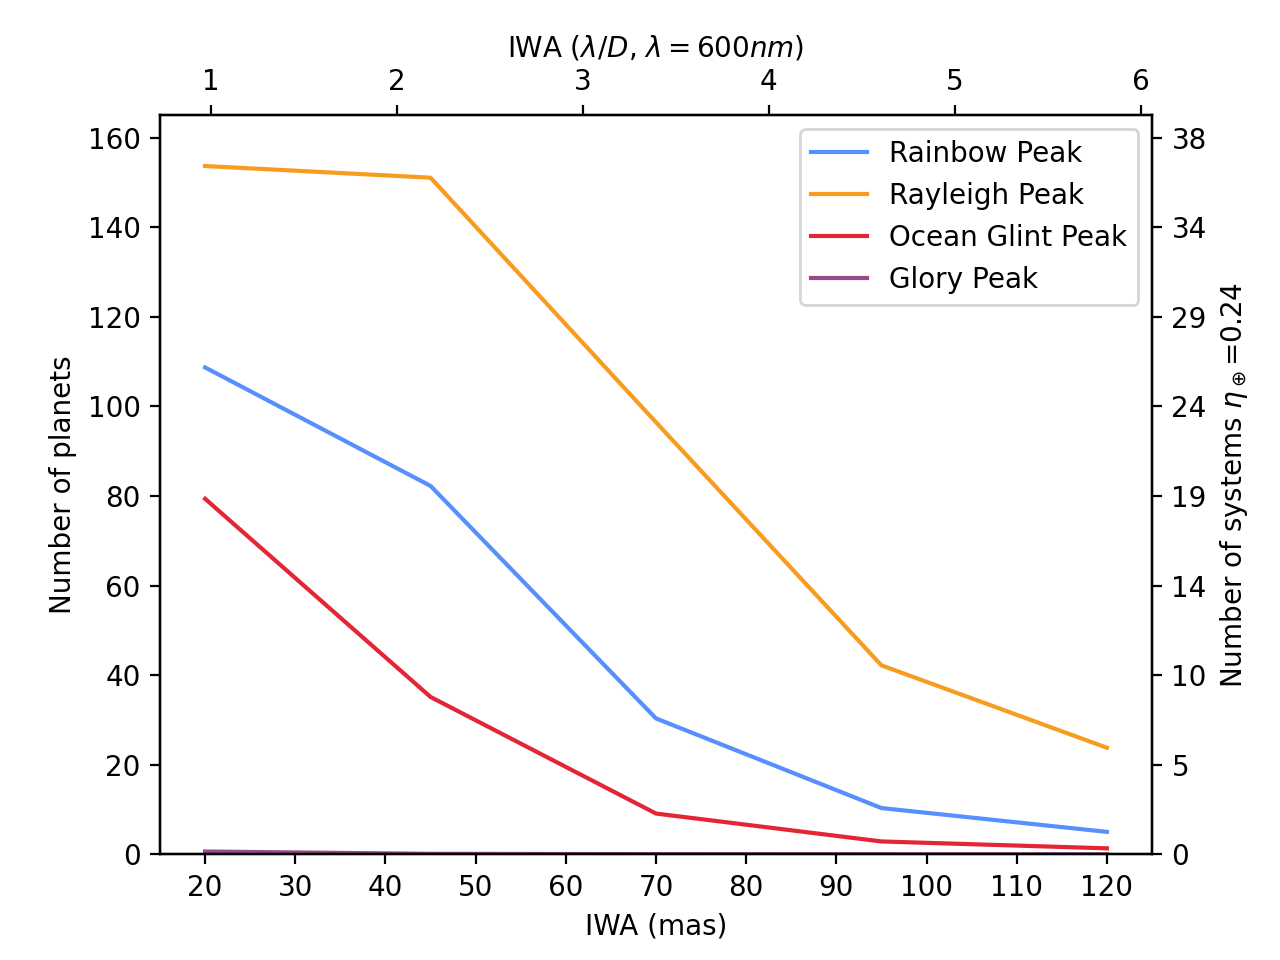
\includegraphics[width=0.6\textwidth]{figures/features_plot_peak.png}  
%    \caption{
%        Number of systems vs inner working angle
%    }
%    \label{fig:accessible_phase_angles}
%\end{figure*}

\begin{figure*}
    \centering
    \includegraphics[width=0.95\textwidth]{figures/nplanets_vs_iwa.png}  
    \caption{
        Number of systems vs inner working angle
    }
    \label{fig:accessible_phase_angles}
    \script{plot_features_vs_iwa.py}
\end{figure*}




%%%%%%%%%%%%%%%%%%%%%%%%%%%%%%%%%%%%%%%%%%%%%%%%%%%%%%%%%%%%%%%

\subsection{The glory of Alpha Cen}%Halelujah
\label{sec:ealpha-cen}
\textbf{Glory science, what it tells us (Kim)}
% Kim will write para on science of glory (what tells us, vaguely why appears here)

%%%%%%%%%%%%%%%%%%%%%%%%%%%%%%%%%%%%%%%%%%%%%%%%%%%%%%%%%%%%%%%

%\subsection{Contrast Curves}
%\label{sec:contrast}

%%%%%%%%%%%%%%%%%%%%%%%%%%%%%%%%%%%%%%%%%%%%%%%%%%%%%%%%%%%%%%%%%%%%%%%%%%%%%%%%%%%%%%%%%%%%%%%%%%%%%%%%%%%%%%%%%%%%%%%%%%%%%%

\section{Conclusions}
%What did we determine? 
%Can we actually detect this stuff for anything in this sample? 
%Do we need to not something about things like A stars which are not included in the sample - they were rejected by the list creators - do we need to comment on this?  - we decided nope.

The Habitable Worlds Observatory is a coronagraphic space mission envisioned to detect and characterise Earth-like exoplanets in the 2040's \todo{check}. 
%
The instrument design and capabilities are still under development and thus can be driven by the science goals of the mission.
%
In this work, we investigated the possibility of using \hwo\ to detect different scattering phenomena which can be used to indicate the habitability of an exoplanet. \todo{more of why this is cool}

Coronagraphy is a rapidly advancing field and it is hard to predict what the capabilities of \hwo\ will be.
%
We primarily focused on the range of scattering phase angles and therefore which scattering phenomena could potentially be observed given the limitation of the coronagraphic \IWA.
%
Assuming a 60 mas \IWA, all of the systems in the NASA Exoplanet Exploration Program's Mission Star List for the Habitable Worlds Observatory would be observable at scattering phases with Rayleigh features, ocean glint would be accessible in $\sim$20 systems, and the rainbows of water clouds in $\sim$55 systems. 
%
The number of systems increases with decreasing \IWA\ and therefore the occurrence rate of Earth-like exoplanets will drive the choice of coronagraphic \IWA\ for this mission.
%
While we briefly considered the contrast ratio of the scattering features, we did not investigate the feasibility of detecting them given their contrast. 
%
This will be an important task once the instrument design and capabilities are better defined and could drive the design of the coronagraph. 


\section*{Software/Data Availability}

The NASA ExEP target list containing the data used for these simulations is available online.% 
\footnote{\url{https://exoplanets.nasa.gov/exep/science-overview/}}
This work has made use of \textsf{numpy}
 \citep{NumPy2020}, \textsf{scipy} \citep{scipy_2020}, \textsf{matplotlib} \citep{matplotlib2007}, and \textsf{astropy},\footnote{\url{https://www.astropy.org}} a community-developed core Python package and an ecosystem of tools and resources for astronomy \citep{astropy:2013, astropy:2018, astropy:2022}.




\section*{Acknowledgements}
The workshop on which this manuscript is based was made possible thanks to the logistical and financial support of the Lorentz Center, Leiden, Netherlands. This workshop was supported by NOVA  and by the European Research Council (ERC) under the European Union's Horizon 2020 research and innovation programme (grant agreement n°866001 - EXACT).

This research has made use of NASA's Astrophysics Data System Bibliographic Services and the SIMBAD database, operated at CDS, Strasbourg, France. 

SRV acknowledges funding from the European Research Council (ERC) under the European Union’s Horizon 2020 research and innovation program under grant agreement No 805445.
SLC acknowledges support from an STFC Ernest Rutherford Fellowship. 
TDG acknowledges funding from the Max Planck ETH Center for Learning Systems.
Specific grant funding and any other specific requirements
KMB acknowledges support from NASA Habitable
Worlds grant No. 80NSSC20K152, and previous support for related work supported by NASA Astrobiology Institute's Virtual Planetary Laboratory under Cooperative Agreement Number NNA13AA93A.

% Add references
\bibliographystyle{mnras}
\bibliography{bib}

\end{document} 